\documentclass{article}
\usepackage[utf8]{inputenc}
\usepackage{fullpage}
\usepackage{amsmath}
\usepackage{hyperref}
\usepackage{amssymb}
\usepackage[most]{tcolorbox}
\usepackage{empheq}
\usepackage{mhchem}
\usepackage{braket}
\usepackage{graphicx}

\newtcbox{\mymath}[1][]{%
    nobeforeafter, math upper, tcbox raise base,
    enhanced, colframe=black!30!black,
    colback=black!30, boxrule=1pt,
    #1}
    
\title{Comp Physics HW5}
\author{Marcus DuPont}
\date{\today}

\begin{document}

\maketitle

\begin{enumerate}
    \item {\textbf{Newman 9.7}\\
    In practice, one utilizes the relaxation method on PDEs, but they can also be extended to ODEs. Take the kinematic problem of projectile motion. We know that the general form of acceleration for said projectile is given by
    \begin{equation*}
        \Ddot{x} = \frac{d^2 x}{dt^2} = - g
    \end{equation*}
    One can rewrite the LHS of this equation to obtain a solution to a good approximation. The ``boundaries'' for this problem are simple the initial and final conditions. The general form for the trajectory is then
    \begin{equation*}
        x(t) = \frac{1}{2}[x(t+\delta t) + x(t-\delta t) + \delta t ^2 g]
    \end{equation*}
    For the exercise, we have the conditions that the ball must be at $x = 0$ in the beginning and after $t = 10 [s]$. From this, we arrive at the following trajectory of the ball (using the relaxation method above).
    \begin{figure}[h!]
        \centering
        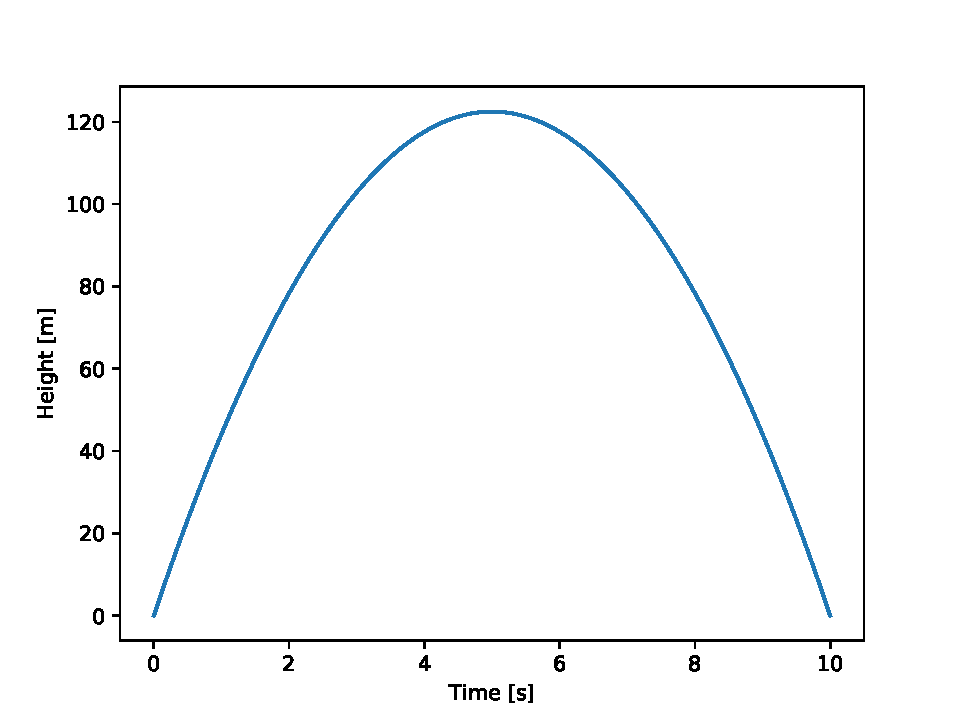
\includegraphics[width=\textwidth, height=9cm]{traj}
        \caption{Trajectory of ball thrown in the air. It reaches a max height of 120 [m] and falls back to its initial position after 10 seconds.}
        \label{fig:my_label}
    \end{figure}
    }
    \item{\textbf{Particles in a Square}:
    \begin{enumerate}
        \item{Taking the particle data given, we can understand how the charge of certain particles might affect their neighbors. To arrive at a charge density grid for these particles, we utilize the `Cloud-in-Cell' method to determine how the charges impact their neighboring cells. The `shape' we can assign these particles are cubes of the form
        \begin{equation*}
            S(x) = \frac{1}{\Delta x}\Pi \left(\frac{x}{\Delta x} \right),
        \end{equation*}
        where $\Delta x$ indicates the spacing between the charges. In our case, since we are working with cells, we will set the cell spacing to 1. The contribution of each particle to the charge in the cell is a sum over all charges within the confined $\Delta x$ cell spacing:
        \begin{equation*}
            W(x_p-x_i) = \int_{x_i - \Delta x/2}^{x_i + \Delta x/2} S(x_p - x)dx
        \end{equation*}
        Here, the index $i$ is the grid index and $p$ is the position of the particle. The total charge density is then
        \begin{equation*}
            \rho = \frac{1}{\Delta x}\sum_{p = 1}^{N_p}m_pW(\pmb{r}_p - \pmb{r}_i)
        \end{equation*}
        \begin{figure}[tp]
            \centering
            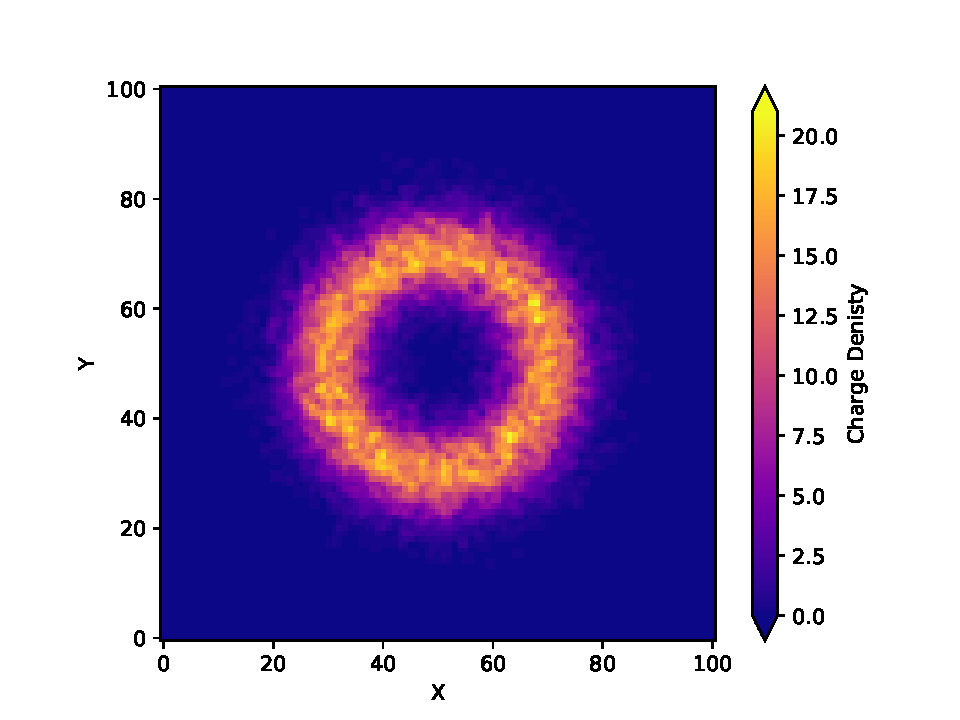
\includegraphics[width=\textwidth, height=9cm]{cahrge_density.pdf}
            \caption{Charge Density grid of given (x,y) coordinates of electron-like particles.}
            \label{fig:my_label}
        \end{figure}
        Luckily, we can simply loop over the particles in a cell and assign charge densities to their neighbors. Since our cell center is located at $\pmb{r}_c = \frac{1}{2}\pmb{r}_p$, we write the relative distance between the particles and the center of the cell as $dr \sim r_p - r_c$. With this, we define a new parameter $t_r := 1- dr$. Doing so allows us to write the density grid values as a linear interpolation
        \begin{equation*}
            \begin{split}
                \rho_{i, j} &= \rho_{i,j} + m_pt_r\\
                \rho_{i+1, j} &= \rho_{i+1,j} + m_pt_r\\
                \vdots\\
                \rho_{i+1, j+1} &= \rho_{i+1, j+1} + m_pt_r
            \end{split}
        \end{equation*}
        Using this method, we arrive at the density plot for this data set.
        }
        \item{Using the relaxation method for the non-static potential, we arrive at its explicit form:
        \begin{equation*}
            \phi(x,y) = \frac{1}{4}(\phi(x+a,y) + \phi(x-a,y) + \phi(x,y+a) + \phi(x,y-a) + \frac{a^2}{\epsilon_0}\rho(x,y))
        \end{equation*}
        Using our charge density we derived in the previous part, we get the potential shown below
        \begin{figure}[tp]
            \centering
            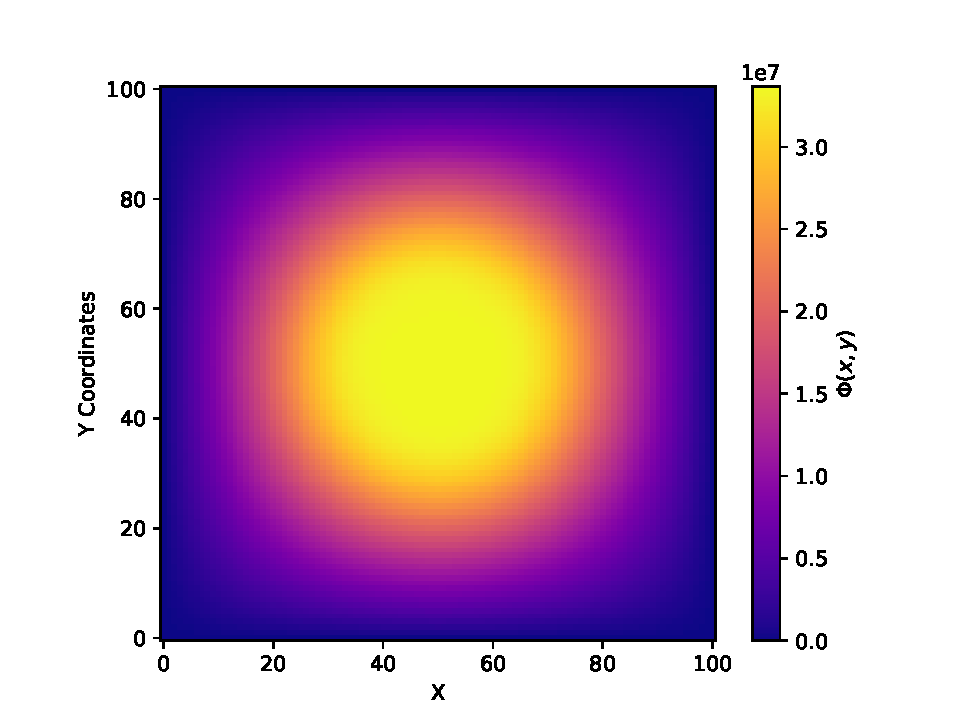
\includegraphics[width=\textwidth, height=9cm]{relaxed_potential_field.pdf}
            \caption{The potential field of the data set using the relaxation method. }
            \label{fig:my_label}
        \end{figure}}
        \item{Lastly, we revisit the potential schema for this problem, but we instead apply the Gauss-Seidel Overrelaxation method for less expensive computation time. This takes the form
        \begin{equation*}
            \phi(x,y) = \frac{1 + \omega}{4}\left[\phi(x+a,y) + \phi(x-a,y) + \phi(x,y+a) + \phi(x,y-a) + \frac{a^2}{\epsilon_0}\rho(x,y) \right] - \omega\phi(x,y)
        \end{equation*}
        Using the Golden Section Search method, we derive an optimal $omega$ valued at 940. Plots of the convergence speed, GS search and potential at the optimal $\omega$ value are shown.
        \begin{figure}[tp]
            \centering
            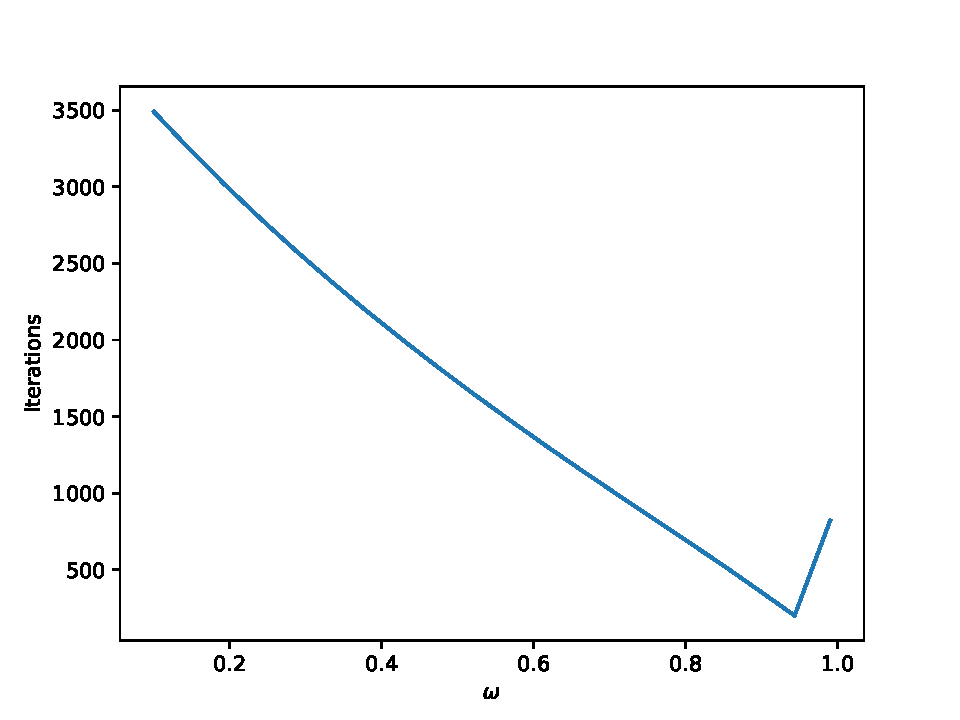
\includegraphics[width=\textwidth, height=8cm]{omega_i.pdf}
            \caption{The required solution iterations for the potential $\phi$ vs the value of $\omega$}
            \label{fig:my_label}
        \end{figure}
        \begin{figure}[h!]
            \centering
            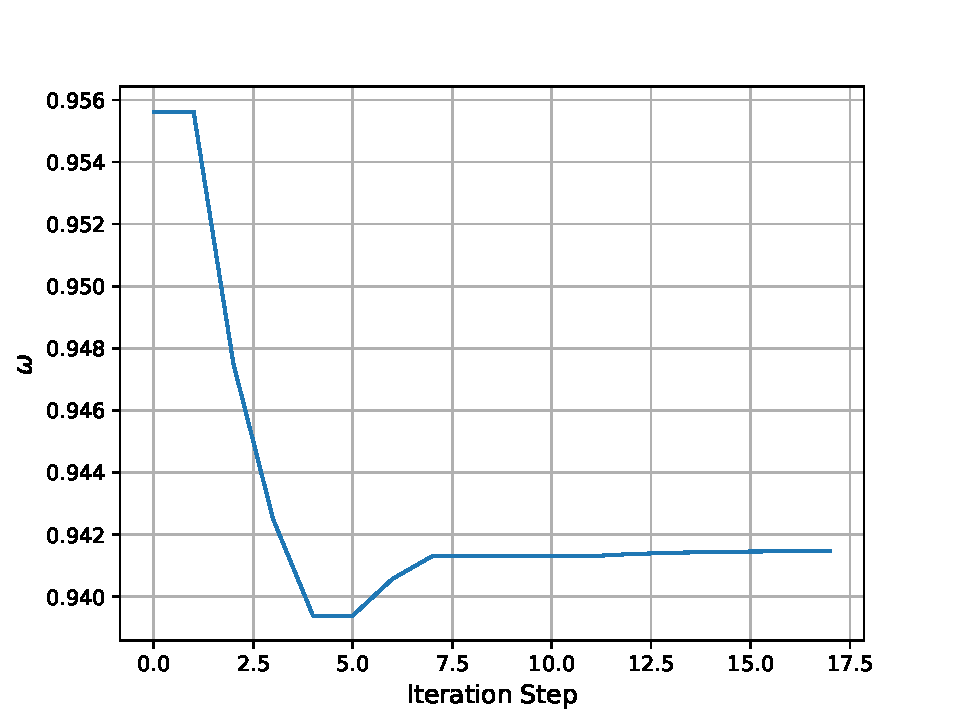
\includegraphics[width=\textwidth, height=8cm]{ratio.pdf}
            \caption{This figures shows how quickly the solution converges depending on how close to the optimal $\omega$ value we are.}
            \label{fig:my_label}
        \end{figure}
        \begin{figure}[htp]
            \centering
            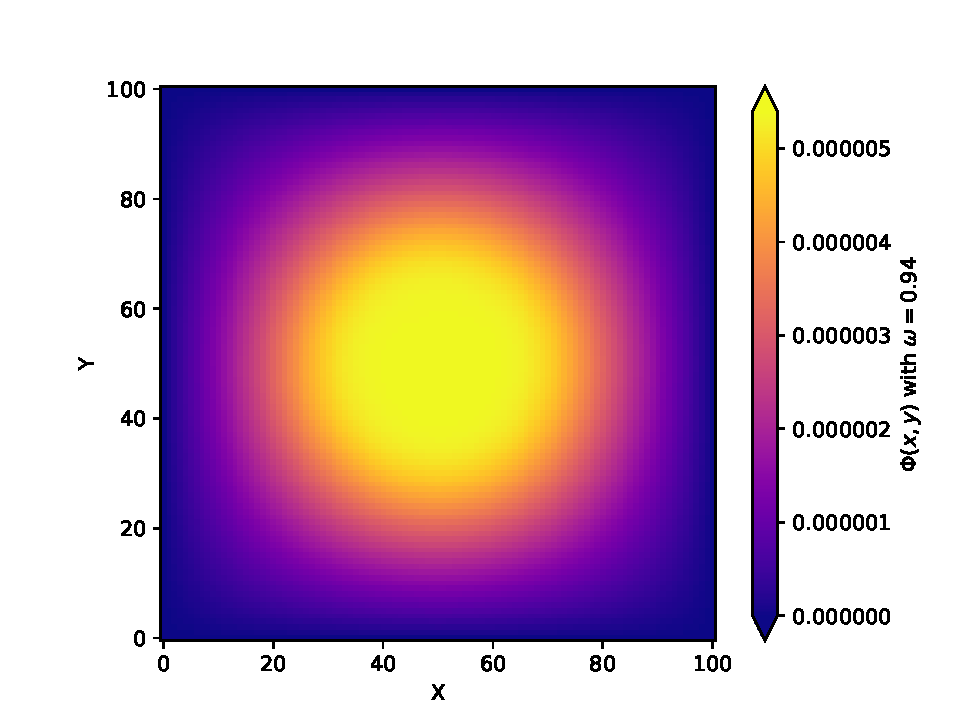
\includegraphics[width=\textwidth, height=8cm]{golden_phi.pdf}
            \caption{The electric potential grid plotted using the optimal $\omega$ value.}
            \label{fig:my_label}
        \end{figure}}
    \end{enumerate}
    }
\end{enumerate}

\end{document}
